\ifajar
  \section{Latihan}
\else
  \section{Bab 2: Browser, HTTP, dan Network Internals}
\fi

Seluruh skrip yang dipakai pada latihan ini tersedia di
\berkas{sources/chapter02/}, dihitung relatif terhadap akar repositori.

\ifajar
  \subsection*{Latihan 1: Profiling dan Penetapan Baseline Performa}
\else
  \subsection*{Prosedur 1: Profiling dan Penetapan Baseline Performa}
\fi

Latihan ini memakai dua halaman situs kampus sebagai objek pengukuran, yaitu
halaman depan \url{https://www.pradita.ac.id} dan satu halaman dalam
\url{https://www.pradita.ac.id/praktisi-akademisi}. Hasil akhirnya adalah catatan angka awal beserta
kondisi pengukurannya.

Satu batasan dipegang sejak awal. Seluruh pengukuran di sini bersifat mengamati,
bukan membebani. Pengukuran dilakukan sebagai satu pengguna biasa memakai
browser dan permintaan tunggal. Uji beban dengan banyak pengguna tiruan,
misalnya memakai k6 seperti pada Listing \ref{lst:k6}, hanya boleh dijalankan
pada sistem milik sendiri atau setelah memperoleh izin tertulis dari pengelola
sistem. Menjalankannya tanpa izin pada situs produksi mengganggu layanan dan
dapat dianggap serangan.

\begin{enumerate}
  \item Buka \texttt{https://www.pradita.ac.id} pada jendela penyamaran, agar
        ekstensi dan \textit{cache} lama tidak memengaruhi hasil.
  \item Buka DevTools, aktifkan Slow 4G dan \textit{throttling} CPU 4 kali lebih lambat,
        lalu muat ulang halaman dengan \textit{cache} dikosongkan.
  \item Catat rincian waktu pada panel Network untuk lima permintaan terlambat,
        beserta pembagian tahapnya.
  \item Rekam panel Performance selama pemuatan halaman, lalu catat seluruh
        \textit{long task} beserta durasinya.
  \item Jalankan Lighthouse pada mode Mobile, lalu catat LCP, INP, dan CLS.
  \item Ukur TTFB memakai \berkas{sources/chapter02/ukur-koneksi.sh}
        seperti pada Listing \ref{lst:curl}. Ulangi 20 kali dengan jeda
        beberapa detik, lalu hitung nilai p50 dan p95 dari hasilnya.
  \item Ulangi langkah 2 sampai 6 pada satu halaman dalam, yaitu
        \url{https://www.pradita.ac.id/praktisi-akademisi}. Halaman itu dipilih
        karena isinya lebih padat daripada halaman depan, sehingga selisih
        angkanya mudah terlihat. Seluruh kondisi pengukuran dijaga sama persis,
        yaitu profil jaringan, faktor \textit{throttling} CPU, dan mode tampilan, agar
        yang dibandingkan benar-benar halamannya, bukan pengaturannya.
  \item Isi \tabisi{tab:baseline} dengan kedua hasil tersebut, lalu
        bandingkan. Perhatikan metrik mana yang berubah paling besar, lalu
        jelaskan penyebabnya berdasarkan bukti dari panel Network dan panel
        Performance.
  \item Isi \tabisi{tab:baseline}, lalu tambahkan satu paragraf berisi
        dugaan penyebab keterlambatan terbesar beserta bukti yang mendasarinya.
\end{enumerate}

\begin{lstlisting}[language=bash, caption={Uji beban dengan k6, tersedia di \berkas{sources/chapter02/skrip-beban.js}, hanya untuk sistem sendiri atau yang sudah berizin}, label={lst:k6}]
k6 run --vus 20 --duration 60s skrip-beban.js
# Catat http_req_duration untuk p(50) dan p(95).
\end{lstlisting}

\ifajar
\begin{table}[!htb]
  \centering
  \caption{Lembar isian baseline performa, diisi untuk dua halaman}
  \label{tab:baseline}
  \begin{tabularx}{\textwidth}{lXcc}
    \hline
    \textbf{Metrik} & \textbf{Cara pengukuran} & \textbf{Halaman depan} & \textbf{Praktisi akademisi} \\
    \hline
    LCP & Lighthouse, mode Mobile & \dots & \dots \\
    \hline
    INP & Lighthouse, mode Mobile & \dots & \dots \\
    \hline
    CLS & Lighthouse, mode Mobile & \dots & \dots \\
    \hline
    TTFB p50 & \texttt{curl}, 20 permintaan & \dots & \dots \\
    \hline
    TTFB p95 & \texttt{curl}, 20 permintaan & \dots & \dots \\
    \hline
    Jumlah aset & DevTools, panel Network & \dots & \dots \\
    \hline
    Total byte & DevTools, panel Network & \dots & \dots \\
    \hline
    Jumlah \textit{long task} & DevTools, panel Performance & \dots & \dots \\
    \hline
  \end{tabularx}
\end{table}
\fi

\ifajar
  \subsection*{Latihan 2: Mengukur Biaya Pembukaan Koneksi}
\else
  \subsection*{Prosedur 2: Mengukur Biaya Pembukaan Koneksi}
\fi

Latihan ini membuktikan bahwa biaya pembukaan koneksi ditentukan oleh jaringan,
bukan oleh kecepatan program di server.

\begin{enumerate}
  \item Jalankan skrip pada Listing \ref{lst:lat1} memakai perintah pada
        Listing \ref{lst:lat1-jalan} untuk tiga domain, yaitu
        \texttt{www.pradita.ac.id}, satu domain kampus di negara tetangga, dan
        satu domain kampus di benua lain.
  \item Skrip tersebut sudah menghitung durasi tiap tahap memakai rumus pada
        Tabel \ref{tab:lat1-rumus}, karena keluaran \texttt{curl} bersifat
        kumulatif sejak permintaan dimulai.
  \item Ambil nilai tengah dari lima pengukuran, lalu isi \tabisi{tab:lat1-hasil} dalam milidetik. Tabel \ref{tab:lat1-contoh}
        memperlihatkan contoh hasil yang sudah terisi.
  \item Jawab tiga pertanyaan berikut. Pertama, berapa persen waktu total yang
        habis sebelum byte pertama tiba? Kedua, tahap mana yang paling besar
        pada tiap domain? Ketiga, apakah domain yang paling jauh selalu paling
        lambat, dan apa penjelasannya?
\end{enumerate}

\begin{lstlisting}[language=bash, caption={Skrip pengukur tiap tahap pembukaan koneksi, tersedia di \berkas{sources/chapter02/ukur-koneksi.sh}}, label={lst:lat1}]
#!/usr/bin/env bash
# Mengukur durasi tiap tahap pembukaan koneksi.
# Pemakaian: ./ukur-koneksi.sh https://www.pradita.ac.id/ [jumlah_ulangan]

url="${1:?alamat wajib diisi}"
ulangan="${2:-5}"

format="%{time_namelookup} %{time_connect} %{time_appconnect}"
format+=" %{time_starttransfer} %{time_total}\n"

printf "%-10s %-10s %-10s %-14s %-10s\n" \
  "DNS" "TCP" "TLS" "TungguServer" "Total"
for ((i = 1; i <= ulangan; i++)); do
  curl -o /dev/null -s -w "$format" --max-time 30 "$url" |
    awk '{
      printf "%-10.0f %-10.0f %-10.0f %-14.0f %-10.0f\n",
        $1*1000, ($2-$1)*1000, ($3-$2)*1000, ($4-$3)*1000, $5*1000
    }'
  sleep 1
done
\end{lstlisting}

Kode di atas tidak perlu diketik ulang. File-nya tersedia pada
\berkas{sources/chapter02/ukur-koneksi.sh}, dihitung relatif terhadap akar
repositori. Jalankan dengan perintah berikut.

\begin{lstlisting}[language=bash, caption={Menjalankan skrip pengukur koneksi}, label={lst:lat1-jalan}]
cd sources/chapter02
./ukur-koneksi.sh https://www.pradita.ac.id/ 5
\end{lstlisting}

\begin{table}[!htb]
  \centering
  \caption{Arti tiap tahap dan cara menghitungnya dari keluaran \texttt{curl}}
  \label{tab:lat1-rumus}
  \begin{tabularx}{\textwidth}{lXX}
    \hline
    \textbf{Tahap} & \textbf{Yang diukur} & \textbf{Rumus} \\
    \hline
    DNS & Lama mencari alamat IP dari nama domain & \texttt{time\_namelookup} \\
    \hline
    TCP & Lama membangun koneksi lewat \textit{three-way handshake} & \texttt{time\_connect} dikurangi \texttt{time\_namelookup} \\
    \hline
    TLS & Lama memeriksa sertifikat dan menyepakati kunci sesi & \texttt{time\_appconnect} dikurangi \texttt{time\_connect} \\
    \hline
    Tunggu server & Lama server memproses permintaan sampai byte pertama keluar & \texttt{time\_starttransfer} dikurangi \texttt{time\_appconnect} \\
    \hline
    Unduh isi & Lama memindahkan sisa isi \textit{response} setelah byte pertama & \texttt{time\_total} dikurangi \texttt{time\_starttransfer} \\
    \hline
  \end{tabularx}
\end{table}

\begin{table}[!htb]
  \centering
  \caption{Contoh hasil yang sudah terisi, dalam milidetik}
  \label{tab:lat1-contoh}
  \begin{tabularx}{\textwidth}{Xccccc}
    \hline
    \textbf{Domain} & \textbf{DNS} & \textbf{TCP} & \textbf{TLS} & \textbf{Tunggu} & \textbf{Total} \\
    \hline
    \texttt{www.pradita.ac.id} & 9 & 46 & 52 & 78 & 188 \\
    \hline
    \texttt{nus.edu.sg} & 9 & 47 & 62 & 36 & 155 \\
    \hline
    \texttt{ethz.ch} & 1 & 39 & 395 & 421 & 855 \\
    \hline
  \end{tabularx}
\end{table}

Contoh pada Tabel \ref{tab:lat1-contoh} sengaja diambil apa adanya, termasuk
kejanggalannya. Domain yang paling jauh memang paling lambat, tetapi tahap TCP
ketiganya justru mirip. Penyebabnya, ketiga situs berada di belakang CDN,
sehingga koneksi berhenti di \textit{edge server} terdekat, sedangkan sisa
perjalanan menuju \textit{origin} baru terasa pada tahap TLS dan tunggu server.
Angka pada tabel tersebut juga bergantung pada lokasi pengukur, sehingga hasil
tiap mahasiswa akan berbeda.

\ifajar
\begin{table}[!htb]
  \centering
  \caption{Lembar isian hasil pengukuran Latihan 2, dalam milidetik}
  \label{tab:lat1-hasil}
  \begin{tabularx}{\textwidth}{Xccccc}
    \hline
    \textbf{Domain} & \textbf{DNS} & \textbf{TCP} & \textbf{TLS} & \textbf{Tunggu} & \textbf{Total} \\
    \hline
    \texttt{www.pradita.ac.id} & \dots & \dots & \dots & \dots & \dots \\
    \hline
    Domain regional: \dots & \dots & \dots & \dots & \dots & \dots \\
    \hline
    Domain antarbenua: \dots & \dots & \dots & \dots & \dots & \dots \\
    \hline
  \end{tabularx}
\end{table}
\fi

\ifajar
  \subsection*{Latihan 3: Membandingkan HTTP/1.1 dan HTTP/2}
\else
  \subsection*{Prosedur 3: Membandingkan HTTP/1.1 dan HTTP/2}
\fi

Latihan ini memperlihatkan pengaruh \textit{multiplexing} pada halaman dengan
banyak aset.

Gambar \ref{fig:devtools-network} memperlihatkan panel Network beserta bagian
yang dipakai pada latihan ini, yaitu kotak centang \emph{Preserve log} dan
\emph{Disable cache} di baris atas, kotak filter di bawahnya, dan baris judul
kolom yang memuat \emph{Name}, \emph{Status}, \emph{Type}, \emph{Initiator},
\emph{Size}, serta \emph{Time}. Baris judul itulah yang diklik kanan untuk
menambahkan kolom \emph{Protocol} dan \emph{Connection ID}.

\begin{figure}[!htb]
  \centering
  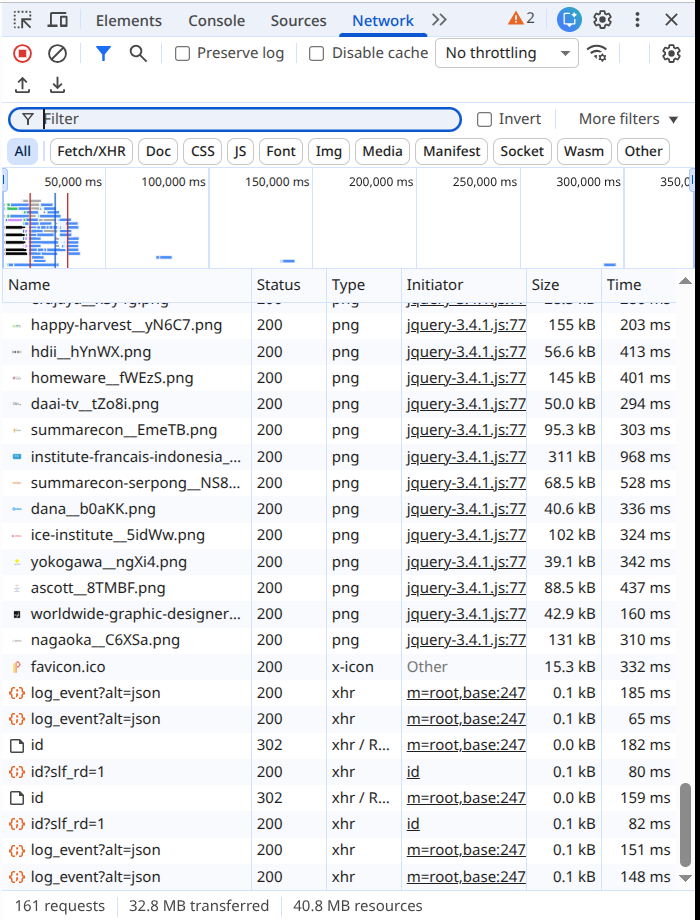
\includegraphics[width=0.72\textwidth, height=0.5\textheight,
                   keepaspectratio]{../figures/devtools-network.png}
  \caption{Panel Network pada Chrome DevTools saat memuat
           \texttt{www.pradita.ac.id}}
  \label{fig:devtools-network}
\end{figure}

\begin{enumerate}
  \item Buka jendela penyamaran, lalu tekan F12 untuk membuka DevTools dan
        pilih panel Network. Panel tersebut hanya merekam selama terbuka,
        sehingga langkah ini dilakukan sebelum halaman dimuat.
  \item Centang \emph{Disable cache} dan \emph{Preserve log}. Tanpa
        \emph{Disable cache}, sebagian besar aset tercatat 0 milidetik, karena
        diambil dari \textit{cache} browser dan tidak menyentuh jaringan sama
        sekali. Cirinya, kolom \emph{Size} menampilkan \emph{(memory cache)}
        atau \emph{(disk cache)}, bukan ukuran byte. Tanpa \emph{Preserve log},
        rekaman terhapus saat terjadi pengalihan, dan
        \texttt{pradita.ac.id} memang mengalihkan ke
        \texttt{www.pradita.ac.id}.
  \item Aktifkan kolom \emph{Protocol} dan \emph{Connection ID}. Kedua kolom
        ini tidak ditampilkan secara bawaan, sehingga harus dipasang sendiri.
        Arahkan penunjuk ke baris judul tabel permintaan, yaitu baris yang
        memuat tulisan \emph{Name}, \emph{Status}, \emph{Type},
        \emph{Initiator}, \emph{Size}, dan \emph{Time}. Klik kanan tepat pada
        baris tersebut, bukan pada baris permintaan di bawahnya, dan bukan pula
        pada bilah alat di atasnya. Menu yang muncul memuat seluruh kolom yang
        tersedia, lengkap dengan tanda centang pada kolom yang sedang aktif,
        seperti terlihat pada Gambar \ref{fig:menu-kolom}. Klik butir
        \emph{Protocol}, lalu ulangi klik kanan dan klik butir \emph{Connection
        ID}. Menu tertutup setiap kali satu butir dipilih, sehingga menyalakan
        dua kolom memang menuntut dua kali klik kanan.

\begin{figure}[!htb]
  \centering
  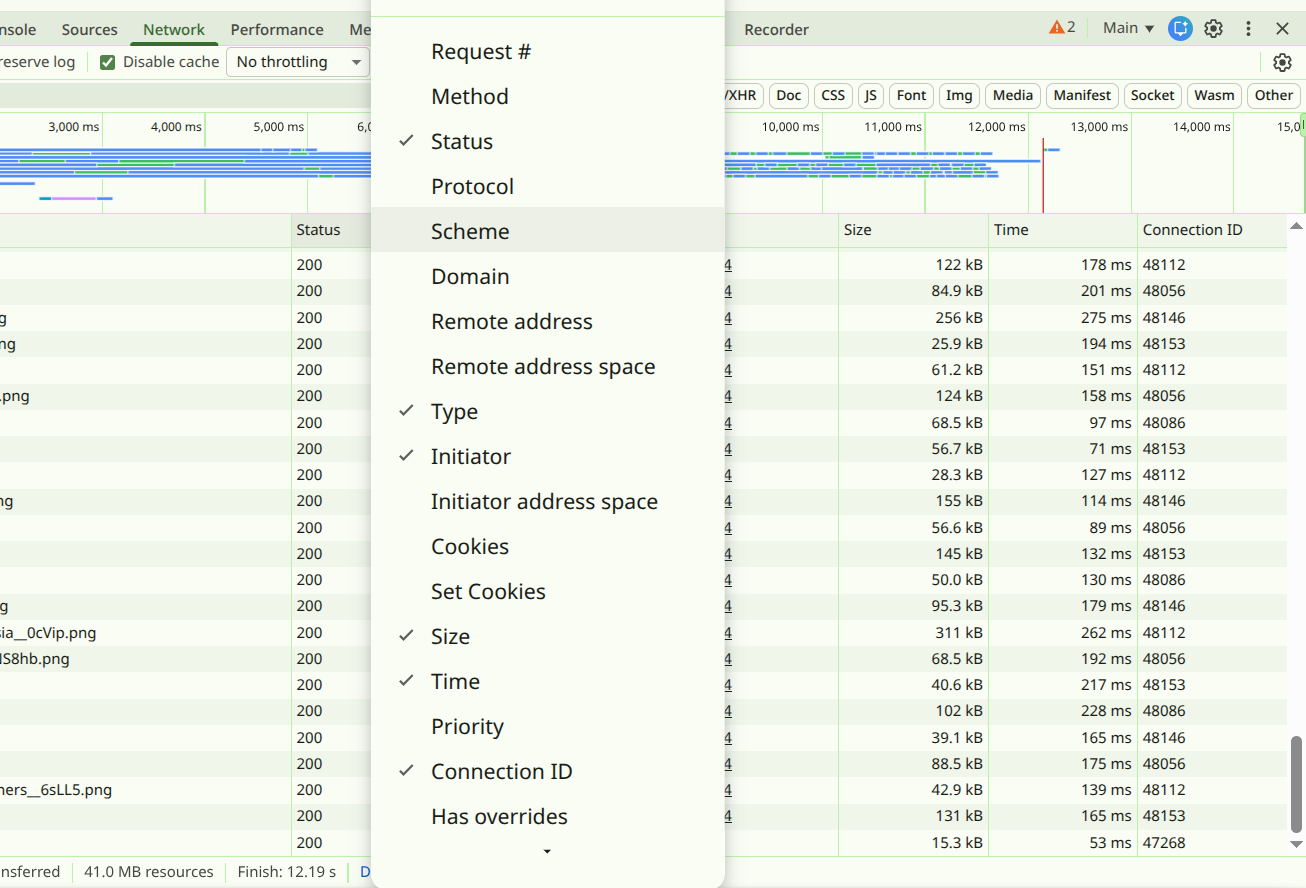
\includegraphics[width=0.68\textwidth, height=0.42\textheight,
                   keepaspectratio]{../figures/devtools-menu-kolom.png}
  \caption{Menu pemilihan kolom yang muncul setelah baris judul tabel
           permintaan diklik kanan. Butir \emph{Protocol} belum tercentang,
           sedangkan \emph{Connection ID} sudah}
  \label{fig:menu-kolom}
\end{figure}

  \item Setelah kedua kolom aktif, tabel permintaan menampilkan versi HTTP dan
        penanda koneksi untuk tiap aset, seperti pada Gambar
        \ref{fig:kolom-koneksi}. Nilai pada kolom \emph{Connection ID} adalah
        nomor soket yang dipakai permintaan tersebut. Nomor yang sama berarti
        permintaan berbagi satu koneksi, sedangkan nomor yang berbeda berarti
        koneksi terpisah. Pada gambar tersebut terlihat beberapa nomor berbeda,
        karena aset halaman berasal dari beberapa host sekaligus.

\begin{figure}[!htb]
  \centering
  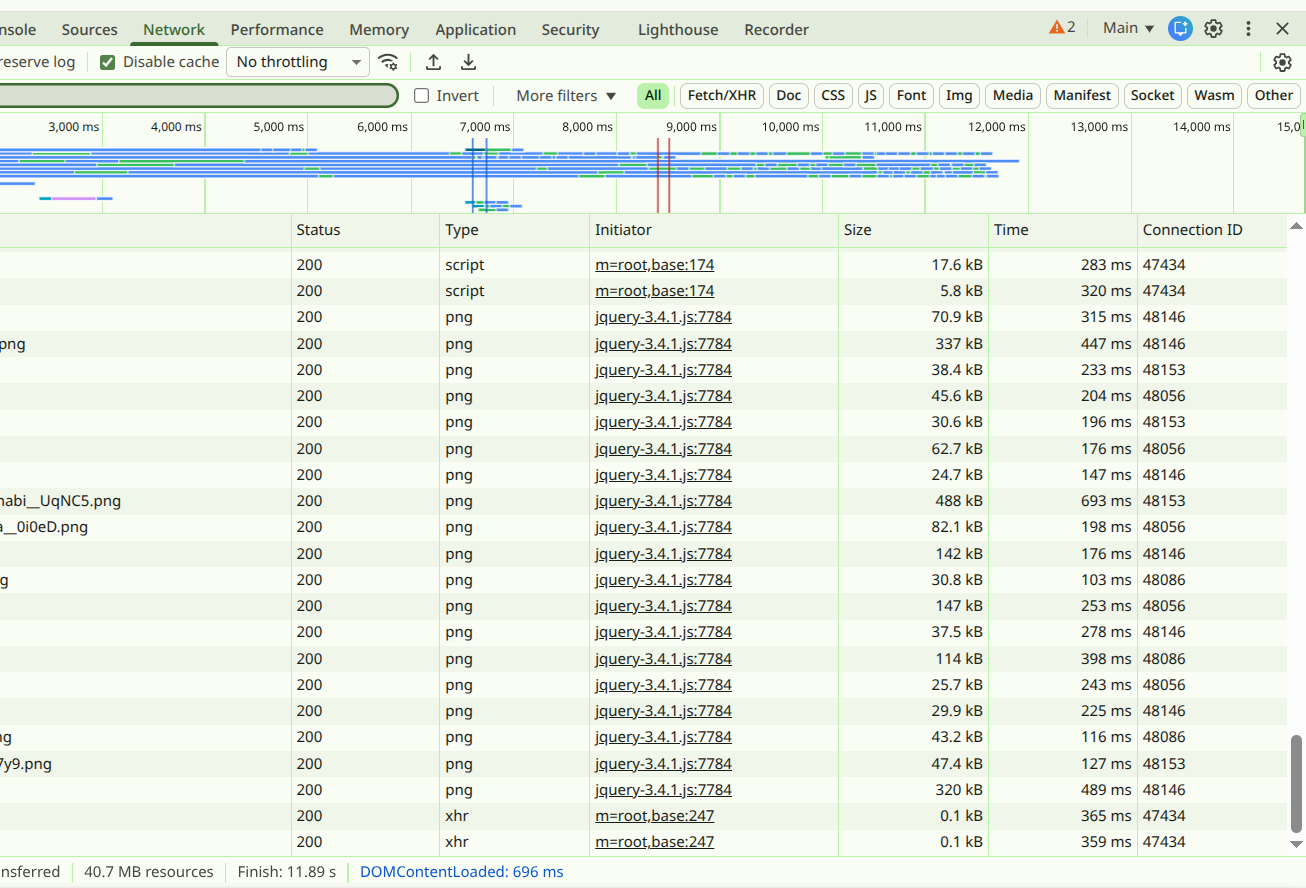
\includegraphics[width=0.68\textwidth, height=0.42\textheight,
                   keepaspectratio]{../figures/devtools-kolom-koneksi.png}
  \caption{Tabel permintaan setelah kolom \emph{Connection ID} diaktifkan.
           Nomor yang sama menandakan permintaan berbagi satu koneksi}
  \label{fig:kolom-koneksi}
\end{figure}

  \item Buka \texttt{aset.txt} yang dihasilkan skrip pada langkah sebelumnya.
        File itu memuat lima alamat aset, misalnya
        \texttt{stylenew.css}, \texttt{stylenewcustom.css},
        \texttt{font-awesome.css}, \texttt{logo\_universitas.png}, dan
        \texttt{Web-Banner-Juli-2019.jpg}.
  \item Ketik nama salah satu file tersebut pada kotak filter di panel
        Network, misalnya \texttt{stylenew.css}. Daftar permintaan akan
        menyusut menjadi baris yang cocok saja. Catat nilai kolom
        \emph{Protocol} dan \emph{Connection ID} pada baris itu, lalu ulangi
        untuk kelima aset. Karena hanya lima, penghitungannya cukup manual.
\ifajar
  \item Isi baris browser pada \tabisi{tab:lat2-hasil} dari catatan
        tersebut. Protokolnya sama untuk kelima aset. Jumlah koneksi dihitung
        dari banyaknya nilai \emph{Connection ID} yang berbeda. Konkurensi
        dilihat dari kolom \emph{Waterfall}, yaitu berapa batang yang mulai
        pada waktu berdekatan. Waktu diambil dari ringkasan \emph{Finish} di
        bagian bawah panel.
\else
  \item Catat hasil pengukurannya.
\fi
  \item Perlu dicatat, pada browser konkurensi tidak dapat ditentukan sendiri.
        Browser yang memutuskan berapa permintaan berjalan bersamaan, dan
        keputusan itu dipengaruhi versi HTTP, prioritas aset, serta batas
        koneksi per host. Karena itu baris browser diisi dengan hasil
        pengamatan, bukan dengan skenario yang dipilih. Peran \texttt{curl}
        justru sebaliknya, yaitu memaksa skenario tertentu agar pengaruh tiap
        faktor dapat dipisahkan.
  \item Perlu dicatat pula, tanpa filter, jumlah permintaan pada browser jauh
        lebih banyak daripada lima aset tersebut. Browser juga memuat dokumen
        HTML-nya sendiri serta file yang baru ketahuan setelah CSS dan
        JavaScript dijalankan. Filter itulah yang menyamakan cakupan
        pengukuran browser dengan pengukuran \texttt{curl}.
  \item Jalankan perintah pada Listing \ref{lst:lat2-jalan}. Skrip tersebut
        mengumpulkan lima alamat aset halaman yang dituju ke
        \texttt{aset.txt}, memeriksa versi HTTP tiap host, lalu mengambil aset
        tersebut dalam empat skenario, yaitu berurutan tanpa pemakaian ulang
        koneksi, berurutan dengan \textit{keep-alive}, serentak di atas
        HTTP/1.1, dan serentak di atas HTTP/2. Secara bawaan hanya aset milik
        host halaman itu sendiri yang diambil. Jumlah koneksi diambil
        dari \texttt{\%\{num\_connects\}} milik \texttt{curl}, sedangkan pada
        browser angka itu terlihat dari banyaknya nilai berbeda pada kolom
        \emph{Connection ID}.
\ifajar
  \item Isi \tabisi{tab:lat2-hasil}. Tabel \ref{tab:lat2-contoh}
        memperlihatkan contoh hasilnya.
\else
  \item Bandingkan hasil pengukuran sendiri dengan Tabel
        \ref{tab:lat2-contoh}.
\fi
  \item Jawab tiga pertanyaan berikut. Pertama, mengapa skenario pertama
        memakai lima koneksi tetapi tetap paling lambat? Kedua, apa yang
        membedakan skenario ketiga dan keempat, padahal konkurensinya sama?
        Ketiga, mengapa jumlah aset tetap penting pada ketiga versi HTTP?
\end{enumerate}

Skrip tersebut memanggil \texttt{kumpulkan-aset.sh} yang juga tersedia pada
direktori yang sama. Jalankan dengan perintah pada Listing
\ref{lst:lat2-jalan}.

Kejadian 0 milidetik tersebut layak diperiksa lebih jauh, karena aset situs
kampus tidak mengirim header \texttt{Cache-Control} maupun \texttt{Expires}.
Yang dikirim hanya \texttt{Last-Modified} dan \texttt{ETag}, seperti terlihat
pada Listing \ref{lst:header-aset}. Dalam keadaan itu browser memakai
\textit{heuristic caching}, yaitu menebak masa berlaku dari umur file. File
yang terakhir diubah lebih dari setahun lalu dianggap masih \textit{fresh} untuk waktu
yang lama, sehingga permintaan berikutnya dilayani dari \textit{cache} tanpa
menghubungi server. Perilaku ini dibahas lebih dalam pada bab \textit{caching},
dan untuk latihan ini cukup dimatikan lewat \emph{Disable cache}.

\begin{lstlisting}[language=bash, caption={Header aset situs kampus, tanpa \texttt{Cache-Control}}, label={lst:header-aset}]
curl -sI https://www.pradita.ac.id/assets/front/css/stylenew.css \
  | grep -iE "cache-control|expires|etag|last-modified"

# Keluarannya:
# last-modified: Fri, 14 Mar 2025 07:37:06 GMT
# etag: "67d3dca2-965"
\end{lstlisting}

\begin{lstlisting}[language=bash, caption={Menjalankan skrip pembanding pada aset milik situs kampus}, label={lst:lat2-jalan}]
cd sources/chapter02
./banding-http.sh https://www.pradita.ac.id/ 5

# Keluarannya:
# Host aset dan versi HTTP yang dilayaninya:
#   www.pradita.ac.id                    HTTP/2    5 aset
#
#   Skenario                            Konkurensi  Koneksi     Waktu
#   1. HTTP/1.1 berurutan, koneksi baru      1         5     2.14 detik
#   2. HTTP/1.1 berurutan, keep-alive        1         1     1.66 detik
#   3. HTTP/1.1 serentak                     5         5     1.92 detik
#   4. HTTP/2 serentak                       5         1     1.87 detik
\end{lstlisting}

\begin{table}[!htb]
  \centering
  \caption{Contoh hasil Latihan 3 yang sudah terisi, lima aset milik
           \texttt{www.pradita.ac.id}}
  \label{tab:lat2-contoh}
  \begin{tabularx}{\textwidth}{Xcccc}
    \hline
    \textbf{Skenario} & \textbf{Aset} & \textbf{Konkurensi} & \textbf{Koneksi} & \textbf{Waktu} \\
    \hline
    HTTP/1.1 berurutan, koneksi baru tiap aset & 5 & 1 & 5 & 2,14 detik \\
    \hline
    HTTP/1.1 berurutan, koneksi dipakai ulang & 5 & 1 & 1 & 1,66 detik \\
    \hline
    HTTP/1.1 serentak & 5 & 5 & 5 & 1,92 detik \\
    \hline
    HTTP/2 serentak & 5 & 5 & 1 & 1,87 detik \\
    \hline
  \end{tabularx}
\end{table}

Empat skenario pada Tabel \ref{tab:lat2-contoh} hanya dapat dipaksakan lewat
\texttt{curl}. Pada browser, keempatnya tidak dapat dipilih, karena browser
sendiri yang menentukan cara mengambil aset. Itulah sebabnya latihan ini memakai
dua alat: \texttt{curl} untuk memisahkan pengaruh tiap faktor, dan browser untuk
melihat perilaku yang sebenarnya terjadi.

Tabel \ref{tab:lat2-contoh} sengaja memisahkan dua hal yang sering tercampur.
Konkurensi berarti berapa permintaan berjalan bersamaan. Koneksi berarti berapa
saluran yang dibuka untuk mencapai konkurensi tersebut. Keduanya tidak selalu
seiring, dan itu terlihat jelas pada empat skenario tersebut.

Dua baris pertama sama-sama berurutan, yaitu permintaan berikutnya baru dikirim
setelah yang sebelumnya selesai. Bedanya hanya pada pemakaian ulang koneksi.
Baris pertama membuka koneksi baru untuk tiap aset, sehingga membayar DNS, TCP,
dan TLS lima kali. Baris kedua memakai satu koneksi untuk lima permintaan
berkat \textit{keep-alive}, dan waktunya turun. Perlu dicatat,
lima koneksi pada baris pertama dibuka bergantian, bukan bersamaan, sehingga
tidak dapat disebut paralel.

Dua baris terakhir barulah paralel, yaitu lima permintaan dikirim bersamaan.
Di sinilah perbedaan kedua versi terlihat. HTTP/1.1 mencapai paralelisme dengan
membuka lima koneksi, sedangkan HTTP/2 mencapainya di dalam satu koneksi lewat
\textit{multiplexing}. Hasil akhirnya mirip, tetapi biayanya berbeda.
Tiap koneksi tambahan menuntut rangkaian pembukaan sendiri dan memakan memori di
kedua sisi. Browser bahkan membatasi jumlahnya sekitar enam per host, sehingga
pada halaman dengan puluhan aset, sisanya harus mengantre.


Satu catatan soal pemilihan aset. Skrip \berkas{kumpulkan-aset.sh} secara
bawaan hanya mengambil aset yang dilayani host halaman itu sendiri. Halaman
kampus sebenarnya juga memuat aset dari domain lain, misalnya penyimpanan objek
dan CDN, dan sebagian di antaranya masih HTTP/1.1. Bila penyaringan tersebut
dimatikan dengan argumen \texttt{semua}, jumlah koneksi pada skenario keempat
akan naik, karena koneksi dihitung per host dan \textit{multiplexing} hanya
berlaku pada host yang mendukung HTTP/2. Hal itu sekaligus menunjukkan biaya
menyebar aset ke banyak domain, sebagaimana dibahas pada Seksi 2.3.
\begin{lstlisting}[language=bash, caption={Memeriksa dukungan HTTP/3 lewat header \texttt{alt-svc}}, label={lst:altsvc}]
curl -sI https://www.pradita.ac.id/ | grep -i alt-svc
# (tidak ada keluaran, berarti HTTP/3 belum diumumkan)

curl -sI https://www.google.com/ | grep -i alt-svc
# alt-svc: h3=":443"; ma=2592000,h3-29=":443"; ma=2592000
\end{lstlisting}


\ifajar
\begin{table}[!htb]
  \centering
  \caption{Lembar isian hasil pengukuran Latihan 3}
  \label{tab:lat2-hasil}
  \begin{tabularx}{\textwidth}{Xcccc}
    \hline
    \textbf{Skenario} & \textbf{Aset} & \textbf{Konkurensi} & \textbf{Koneksi} & \textbf{Waktu} \\
    \hline
    Browser, dibaca dari kolom \emph{Protocol} dan \emph{Connection ID} & 5 & \dots & \dots & \dots \\
    \hline
    HTTP/1.1 berurutan, koneksi baru tiap aset & 5 & 1 & \dots & \dots \\
    \hline
    HTTP/1.1 berurutan, koneksi dipakai ulang & 5 & 1 & \dots & \dots \\
    \hline
    HTTP/1.1 serentak & 5 & 5 & \dots & \dots \\
    \hline
    HTTP/2 serentak & 5 & 5 & \dots & \dots \\
    \hline
  \end{tabularx}
\end{table}
\fi

Pertanyaan berikutnya, mengapa HTTP/3 tidak ikut diukur. Ada dua alasan yang
keduanya dapat diperiksa sendiri. Pertama, \texttt{curl} bawaan Ubuntu tidak
dibangun dengan dukungan HTTP/3, sehingga opsi \texttt{--http3} ditolak dengan
pesan \emph{the installed libcurl version doesn't support this}. Dukungan itu
menuntut \texttt{libcurl} yang dibangun bersama pustaka QUIC seperti ngtcp2 atau
quiche, dan pembangunan tersebut di luar cakupan bab ini. Kedua,
\texttt{www.pradita.ac.id} sendiri belum menyediakan HTTP/3. Hal itu dapat
diperiksa tanpa mengunduh apa pun, yaitu lewat header \texttt{alt-svc} pada
\textit{response}, seperti pada Listing \ref{lst:altsvc}. Pada browser, versi yang
benar-benar dipakai terlihat pada kolom \emph{Protocol}, dengan nilai
\texttt{h2} untuk HTTP/2 dan \texttt{h3} untuk HTTP/3.



Angka waktu berubah tiap kali pengukuran dijalankan, karena bergantung pada
kondisi jaringan dan beban server. Yang perlu dilaporkan adalah pola
perbandingannya beserta penjelasannya, bukan angka persisnya.

